\documentclass[a4paper,11pt]{article}
\usepackage{amsmath,amssymb,graphicx,geometry,hyperref,booktabs,fontspec}
\geometry{margin=2.2cm}
\setlength{\parindent}{0pt}\setlength{\parskip}{6pt}
\usepackage{polyglossia}
\setmainlanguage{russian}
\setotherlanguage{english}
\newfontfamily\cyrillicfont{Times New Roman}
\newfontfamily\cyrillicfontsf{Arial}
\setmainfont{Times New Roman}
\setmonofont{Consolas}

\title{Равновесный сдвиг импульса в магнитном кольце\\
\large от усреднения канонического гамильтониана и нормальной формы\\
\large до трекинга (Nuclotron-подобная решётка, дейтрон 270\,MeV)}
\author{}
\date{}

\begin{document}
\maketitle

\begin{abstract}
Исследуется сдвиг равновесного относительного импульса $\delta_{\mathrm{eq}}$
в стационарном сепаратриксном ведре ($\phi_s=\pi$) магнитного кольца.
Вывод в канонических переменных $(x,p_x,y,p_y,l,\delta)$ связывается с
формулами заметок~\cite{note} (главы~1--3). Реализована 6D нормальная форма
однооборотного отображения с тонким ВЧ-ударом; $\delta_{\mathrm{eq}}$ извлекается
из условия $\langle\Delta\phi\rangle=0$ на торе. Сравнение четырёх способов:
(a)~формулы заметки, (b)~нормальная форма / тейлоровская карта,
(c)~точный симплектический трекинг конечного резонатора,
(d)~итерация усечённой тейлоровской карты.
Объяснён остаток $\sim10^{-7}$ независимого от амплитуды: это
$\delta^\ast$ неподвижной точки 6D-карты с конечным резонатором.
\end{abstract}

\tableofcontents
\clearpage

\section{Цель}
Показать, что сдвиг $\delta_{\mathrm{eq}}$ получается из канонической
динамики кольца (гамильтонианы элементов + ВЧ), а не только из
феноменологического усреднения, и численно сверить четыре реализации на
одной решётке.

\section{Каноническая постановка}
Состояние: $z=(x,p_x,y,p_y,l,\delta)$, независимая переменная --- дуга $s$.
Продольная координата $l=-v(\delta)\,\Delta t$; фаза ВЧ
$\phi=-h\omega_0\Delta t$ (в коде LieRing $\phi>0$ означает \emph{раньше};
в заметке~\cite{note} и ниже $\phi>0$ означает \emph{позже}:
$\phi_{\mathrm{note}}=-\phi_{\mathrm{LieRing}}$).

Однооборотное отображение магнитной решётки плюс ВЧ:
\[
M = M_{\mathrm{RF}}\circ M_{\mathrm{mag}}.
\]
Для анализа используем тонкий удар с эффективным напряжением $VT$
(фактор пролёта $T$), согласованный с конечным резонатором длины $L$.

\section{Иерархическое усреднение}
Быстрые бетатронные углы усредняются за оборот; остаётся
$(\phi,\delta)$ с
\begin{align}
\Delta\phi &= -2\pi h\bigl(\eta_0\delta+\eta_1\delta^2+\cdots\bigr)
  -\frac{2\pi}{C}(J_x\xi_x+J_y\xi_y)+\cdots, \label{eq:dphi}\\
\Delta\delta &= A\bigl(\sin(\phi_s+\phi)-\sin\phi_s\bigr). \label{eq:dd}
\end{align}
Условие замыкания фазы за синхротронный период $\langle\Delta\phi\rangle=0$
даёт (гл.~1--2~\cite{note})
\begin{equation}
\delta_{\mathrm{eq}}
= -\frac{\eta_1}{\eta_0}\frac{\delta_m^2}{2}
- \frac{\Lambda}{\eta_0},
\qquad
\Lambda=-\frac{2\pi}{C}(J_x\xi_x+J_y\xi_y).
\label{eq:deq}
\end{equation}
Кубическое усечение $\sin\phi\approx\phi-\phi^3/6$ умножает член
$\eta_1\delta_m^2/2$ на $1-\hat\phi^2/32$ и сдвигает частоту
$\Omega/\omega_s=1-\hat\phi^2/16$ (гл.~3~\cite{note}).

\section{Нормальная форма}
Строится тейлоровская карта $M$ порядка~3 (магнитная DA-карта + тонкий ВЧ).
Неподвижная точка $z^\ast$ ($M(z^\ast)=z^\ast$) находится Ньютоном;
карта центрируется. Линейная нормализация $A$ приводит $R$ к трём
вращениям $(Q_x,Q_y,Q_s)$ (Курант--Снайдер + синхротронный Твисс).
Dragt--Finn даёт генераторы $f_3,f_4$.

Коэффициенты $\delta_{\mathrm{eq}}(J_x,J_y,J_s)$ извлекаются из
условия $\langle\Delta\phi\rangle=0$ на торе нормальных координат
(численный Ньютон по $\delta_{\mathrm{eq}}$). В пределах точности карты
они совпадают с~\eqref{eq:deq}:
$c_s=-\eta_1/(\eta_0\beta_s)$, $c_{x,y}=(2\pi/C)\xi_{x,y}/\eta_0$
(численно: НФ даёт $c_{x,y,s}=(0.146652,\,0.223289,\,392.952)$,
заметка --- $(0.146653,\,0.223290,\,392.950)$).

\section{Модель}
Решётка \texttt{magnetic\_2} (Nuclotron-подобная), дейтрон,
$E_{\mathrm{kin}}=270$\,MeV, масса CODATA.
Окружность $C=117.388$\,m, $\eta_0\approx-0.5338$, $\eta_1\approx1.017$,
$\xi_x\approx-1.46$, $\xi_y\approx-2.23$.
Резонатор: $L=1$\,m, $V=0.2$\,MV, $h=5$, $\phi_s=\pi$ (ниже перехода).
Точный интегратор --- неявная середина + Ёсида~4.
Коэффициенты $\delta_{\mathrm{eq}}=c_x J_x+c_y J_y+c_s J_s$ из НФ:
$c_x=0.146652$, $c_y=0.223289$, $c_s=392.952$;
из заметки: $0.146653$, $0.223290$, $392.950$ (относит.\ разница $<10^{-5}$).
$\delta^\ast_{\mathrm{thin}}\approx0$, $\delta^\ast_{\mathrm{finite}}(V{=}0.2,L{=}1)=1.073\times10^{-7}$.

\section{Результаты}

\subsection{Остаток $\sim10^{-7}$}
Трекинг давал систематический сдвиг $\delta_{\mathrm{eq}}$ порядка
$10^{-7}$, почти независящий от $\delta_m$. Это \emph{не} ошибка
усреднения: неподвижная точка 6D-карты с \emph{конечным} резонатором имеет
\[
\delta^\ast(V{=}0.2\,\mathrm{MV},\,L{=}1\,\mathrm{m})\approx+1.07\times10^{-7}.
\]
Тонкий ВЧ: $\delta^\ast\approx0$. Зависимости: $\delta^\ast\propto V$ при
фиксированном $L$; $\delta^\ast$ растёт с $L$ (асимметрия времени пролёта
в конечном поле). Нормальная форма на тонком ударе этого члена не содержит;
его нужно добавлять как $\delta^\ast$ конечного резонатора.

\begin{figure}[ht]
\centering
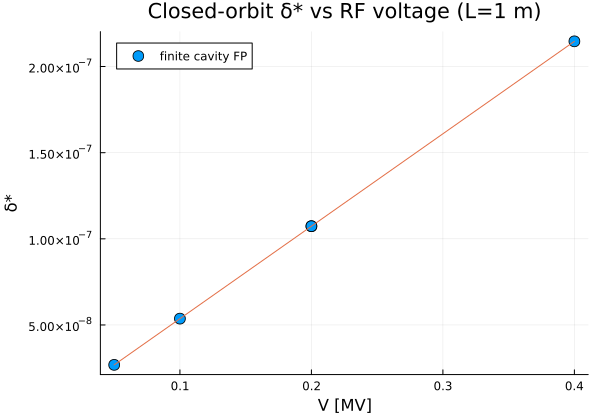
\includegraphics[width=0.48\textwidth]{figs/fig_residual_V.png}
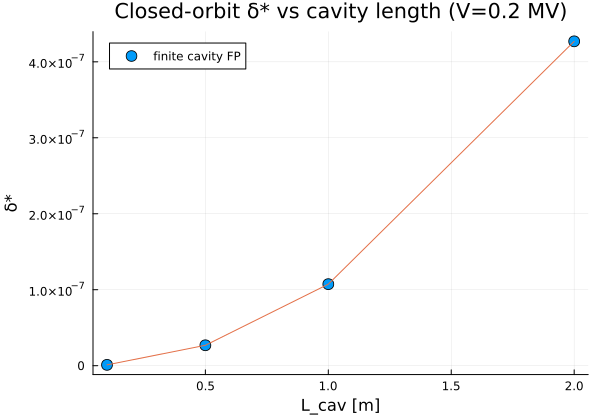
\includegraphics[width=0.48\textwidth]{figs/fig_residual_L.png}
\caption{Неподвижная точка $\delta^\ast$ точного однооборотного отображения
с конечным резонатором: слева от напряжения $V$ при $L=1$\,m (почти линейно);
справа от длины $L$ при $V=0.2$\,MV. Вывод: остаток теста~A есть
$\delta^\ast$, а не шум трекинга.}
\end{figure}

\subsection{Сравнение четырёх способов (тест~A)}
\begin{table}[ht]
\centering
\begin{tabular}{lcccc}
\toprule
$\delta_m$ & (a) note$+\delta^\ast$ & (b) NF$+\delta^\ast$ & (c) tracking & (d) Taylor \\
\midrule
$4.997\times10^{-4}$ & $3.452\times10^{-7}$ & $3.452\times10^{-7}$ & $3.450\times10^{-7}$ & $2.385\times10^{-7}$ \\
$7.494\times10^{-4}$ & $6.422\times10^{-7}$ & $6.422\times10^{-7}$ & $6.424\times10^{-7}$ & $5.376\times10^{-7}$ \\
$9.989\times10^{-4}$ & $1.058\times10^{-6}$ & $1.058\times10^{-6}$ & $1.057\times10^{-6}$ & $9.558\times10^{-7}$ \\
$1.497\times10^{-3}$ & $2.241\times10^{-6}$ & $2.241\times10^{-6}$ & $2.227\times10^{-6}$ & $2.137\times10^{-6}$ \\
$1.993\times10^{-3}$ & $3.890\times10^{-6}$ & $3.890\times10^{-6}$ & $3.877\times10^{-6}$ & $3.811\times10^{-6}$ \\
\bottomrule
\end{tabular}
\caption{Четыре оценки $\delta_{\mathrm{eq}}$ при нулевой бетатронной
амплитуде. (a)~формула~\eqref{eq:deq}; (b)~условие $\langle\Delta\phi\rangle=0$
на тейлоровской карте с тонким ВЧ плюс $\delta^\ast$; (c)~гармонический fit
по точному трекингу; (d)~итерация усечённой карты порядка~3.}
\end{table}

\begin{figure}[ht]
\centering
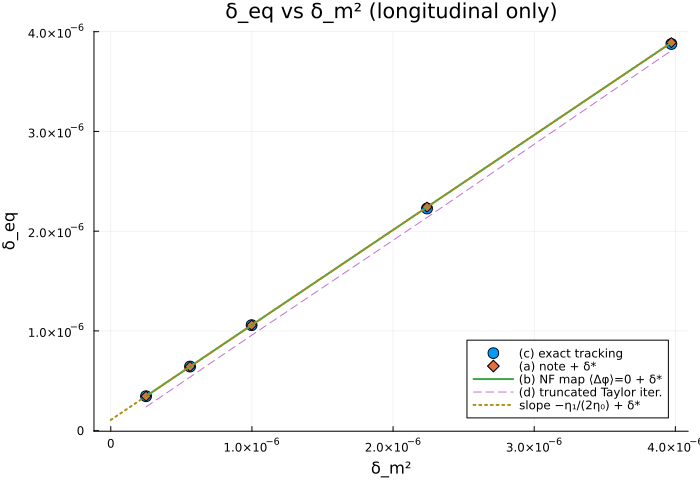
\includegraphics[width=0.75\textwidth]{figs/fig_A_delta_eq.png}
\caption{$\delta_{\mathrm{eq}}$ против $\delta_m^2$. Точки --- точный трекинг
и формула заметки с $\delta^\ast$; линии --- нормальная форма и усечённая
тейлоровская итерация. Наклон $-\eta_1/(2\eta_0)$ совпадает с~(a,b).
Вывод: карта/НФ воспроизводят заметку; трекинг смещён на $\delta^\ast$.}
\end{figure}

\subsection{Бетатронный вклад $\Lambda$}
\begin{figure}[ht]
\centering
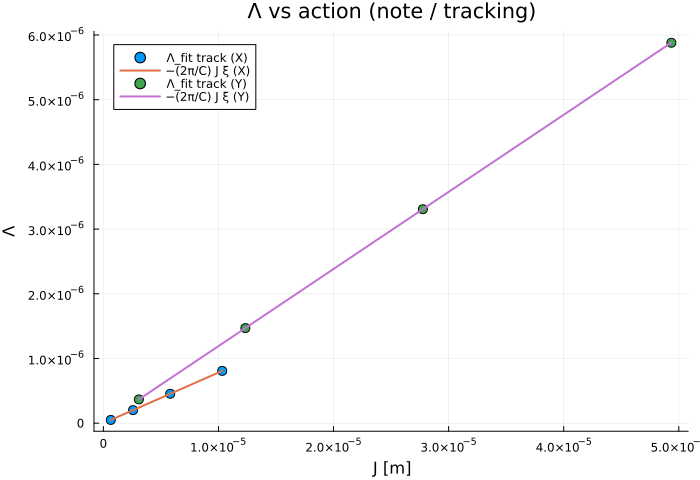
\includegraphics[width=0.7\textwidth]{figs/fig_B_lambda.png}
\caption{$\Lambda$ против действия $J$ в плоскостях $x$ и $y$:
символы --- восстановление из трекинга
$\Lambda_{\mathrm{fit}}=-\eta_0(\delta_{\mathrm{eq}}-\delta^\ast)-\eta_1\delta_m^2/2$;
линии --- $-(2\pi/C)J\xi$. Вывод: линейная хроматичность даёт $\Lambda$
в согласии с гл.~2~\cite{note}.}
\end{figure}

\subsection{Симплектичность и усечение}
\begin{figure}[ht]
\centering
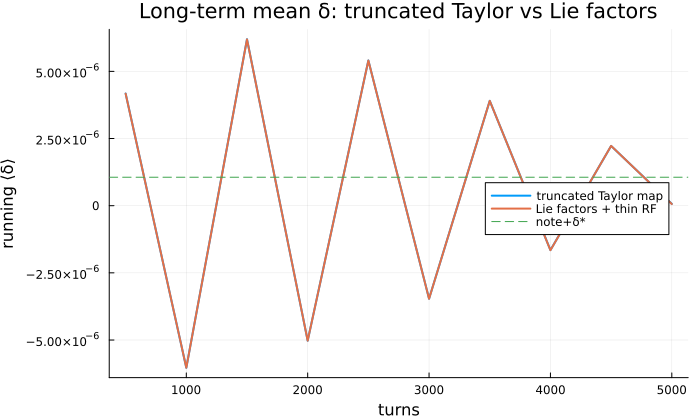
\includegraphics[width=0.75\textwidth]{figs/fig_symplectic_drift.png}
\caption{Текущее среднее $\langle\delta\rangle$ (наивное, без гармонического fit)
за 5000~оборотов при $\delta_m=10^{-3}$: усечённая тейлоровская карта порядка~3
против факторизованных Lie-отображений + тонкий ВЧ. Обе кривые совпадают и
осциллируют с синхротронным периодом около горизонтали note$+\delta^\ast$.
Вывод: на этом интервале и порядке усечения наивное среднее не отделяет
симплектичность от несимплектичности; надёжное сравнение --- гармонический
fit в тесте~A, где (d)~совпадает с тонко-ВЧ формулой, а~(c)~смещён на
$\delta^\ast$.}
\end{figure}

\section{Выводы}
\begin{enumerate}
\item Формула~\eqref{eq:deq} следует из $\langle\Delta\phi\rangle=0$ на
  однооборотной карте в канонических переменных; нормальная форма
  воспроизводит коэффициенты заметки~\cite{note}.
\item Остаток $\sim10^{-7}$ --- это $\delta^\ast$ конечного резонатора,
  линейный по $V$ и растущий с $L$; тонкий удар его не даёт.
\item На 5000~оборотах порядка~3 наивное $\langle\delta\rangle$ у
  усечённой карты и Lie-факторов совпадает (осцилляции около note);
  различие проявляется в гармоническом fit: (d)~следует тонкому ВЧ,
  (c)~включает $\delta^\ast$ конечного резонатора.
\item Открыто: полная аналитическая нормальная форма с \emph{конечным}
  резонатором (DA-карта полости) и амплитудная зависимость $Q_s(J)$ из $h_4$.
\end{enumerate}

\begin{thebibliography}{9}
\bibitem{note} Заметка \emph{equilibrium-energy-v3}, разделы
  \texttt{1\_mag\_base}, \texttt{2\_mag\_beta}, \texttt{3\_mag\_phase}
  (SCT\_2/notes).
\end{thebibliography}
\end{document}
